% tex for data

\documentclass{article}
\usepackage{url,graphicx,tabularx,array,amsmath,amssymb,amsthm,booktabs,float}
\usepackage[margin=.65in]{geometry}
\usepackage[toc,page]{appendix}
\graphicspath{{C:/Users/Colin/Documents/GitHub/533-proj/}{C:\Users}}
\begin{document}
\noindent \textit{Data:}\\\\
The data analyzed is hard drive testing data from the company, Backblaze.  Since 2013, Backblaze has been continuously spinning hard drives in controlled storage pods.  Hard drives are run till they fail or are right censored.  When a hard drive fails it is permanently removed from testing.  In addition, new hard drives are regularly added to the testing sample.  The latest data provided by Backblaze goes from January 1, 2015 to September 30, 2015.  Blackblaze provides over 70 variables on each hard drive; we wll focus on the following subset: an indicator variable for the last day the hard drive was in service before failing, the number of hours a hard drive has been on test, and the model/brand of each hard drive.\\\\
The raw data download from Backblaze contained 54,398 unique drives.  Before analyzing the data, however, we removed certain observations.  Any models with fewer than 100 drives in testing were excluded.  Also, drives that failed in fewer than 20 days were removed.  There were some other bizarre observations in the data; for example, hard drives listed as being in test for over 10 years or drives that entered and exited the sample on the same day.  These bizarre observations were likely due to mis-coding and were dropped.  After cleaning the data we had a sample size of 52,811 total drives for analysis.\\\\
The final sample included 21 hard drive models.  Below is a summary of the distribution of failures, and total testing time for each model.  The total number of failures was 1030.  The majority of those failures came from models 5, 7, 9, and 11.  Not surprising, model 11, which had the most failures also had the longest total testing time; however, this relationship was not uniform across models.  Model 1 had the 2nd longest total testing time, but relatively few failures.
\begin{figure}[H]
\centering
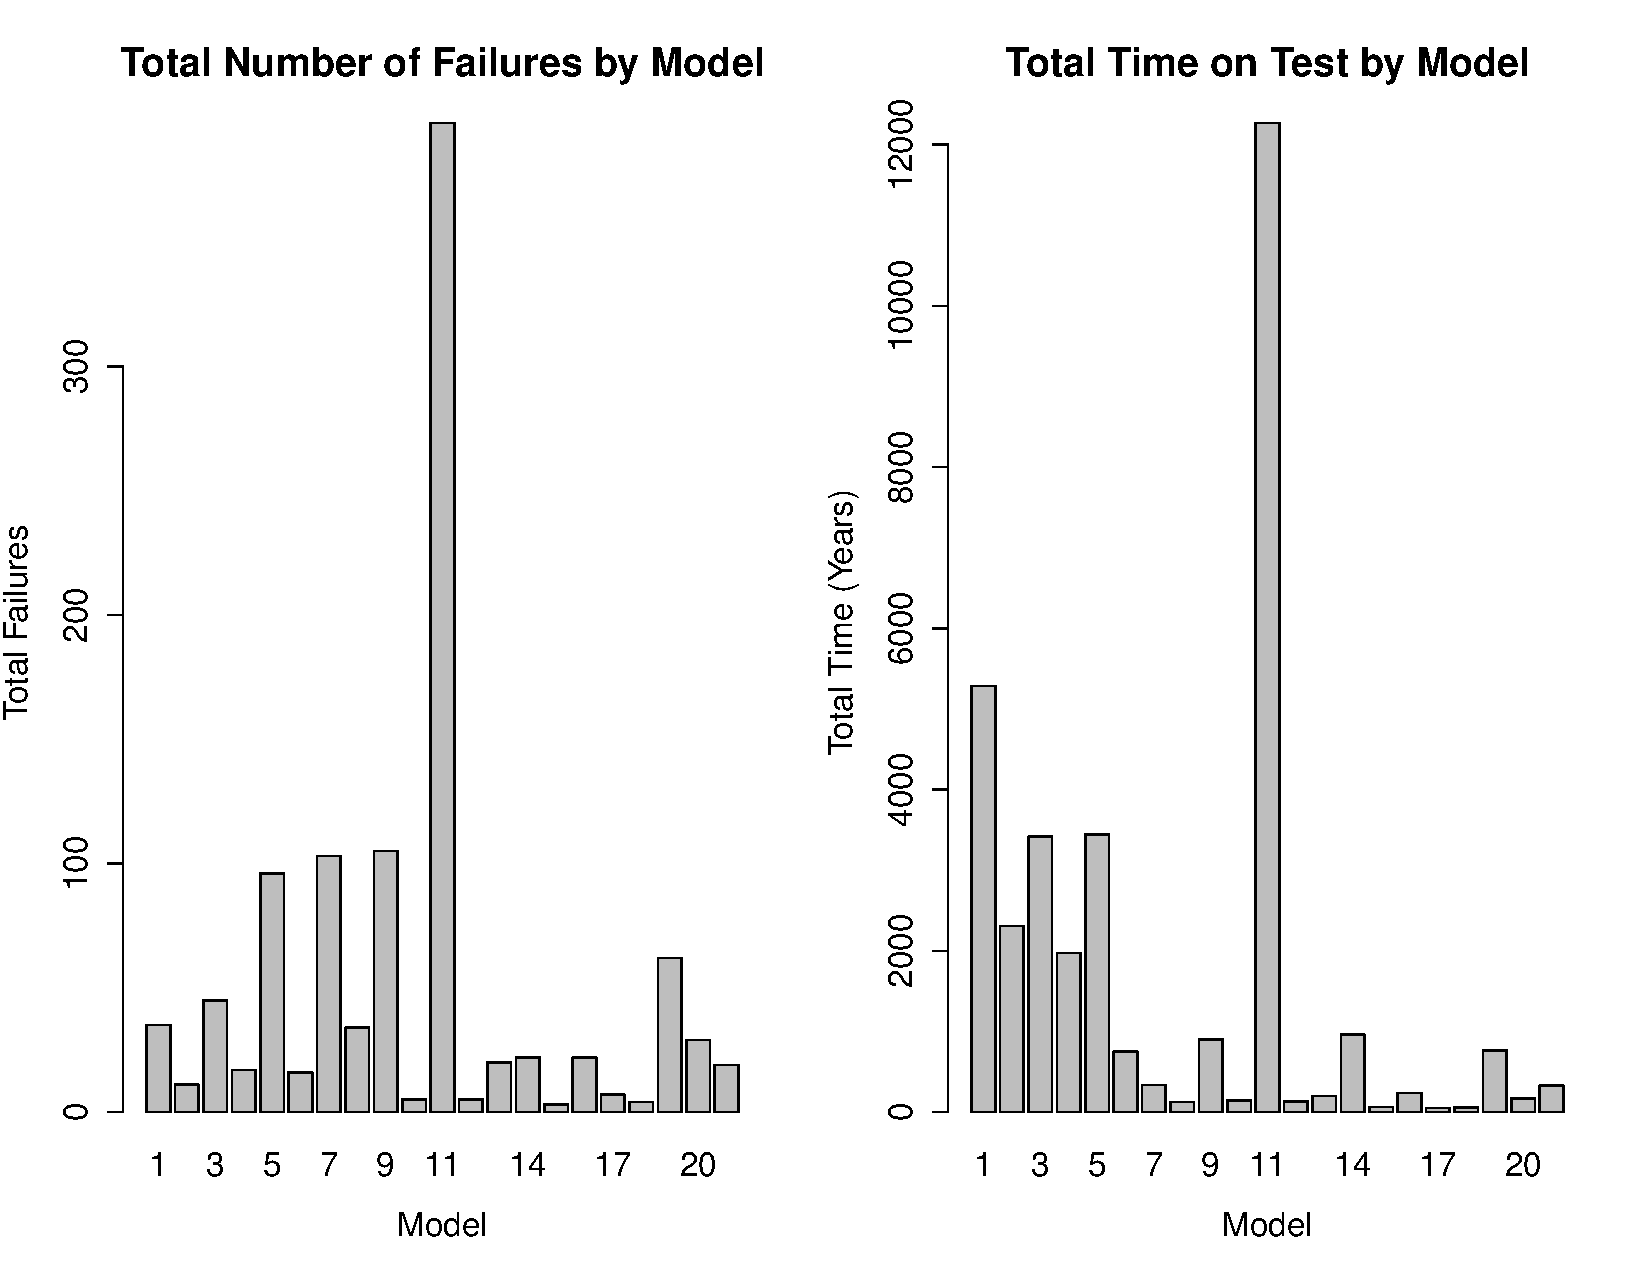
\includegraphics[height=10cm]{sumstat1.pdf}
\end{figure}
\noindent We also examined the distribution of failure times.  The shape is slightly skewed to the right with the majority of failures occurring within 250 days. However, with over 50,000 of the hard drives start times left truncated it is specious to infer that the failire times suffer from infant mortality.   
\begin{figure}[H]
\centering
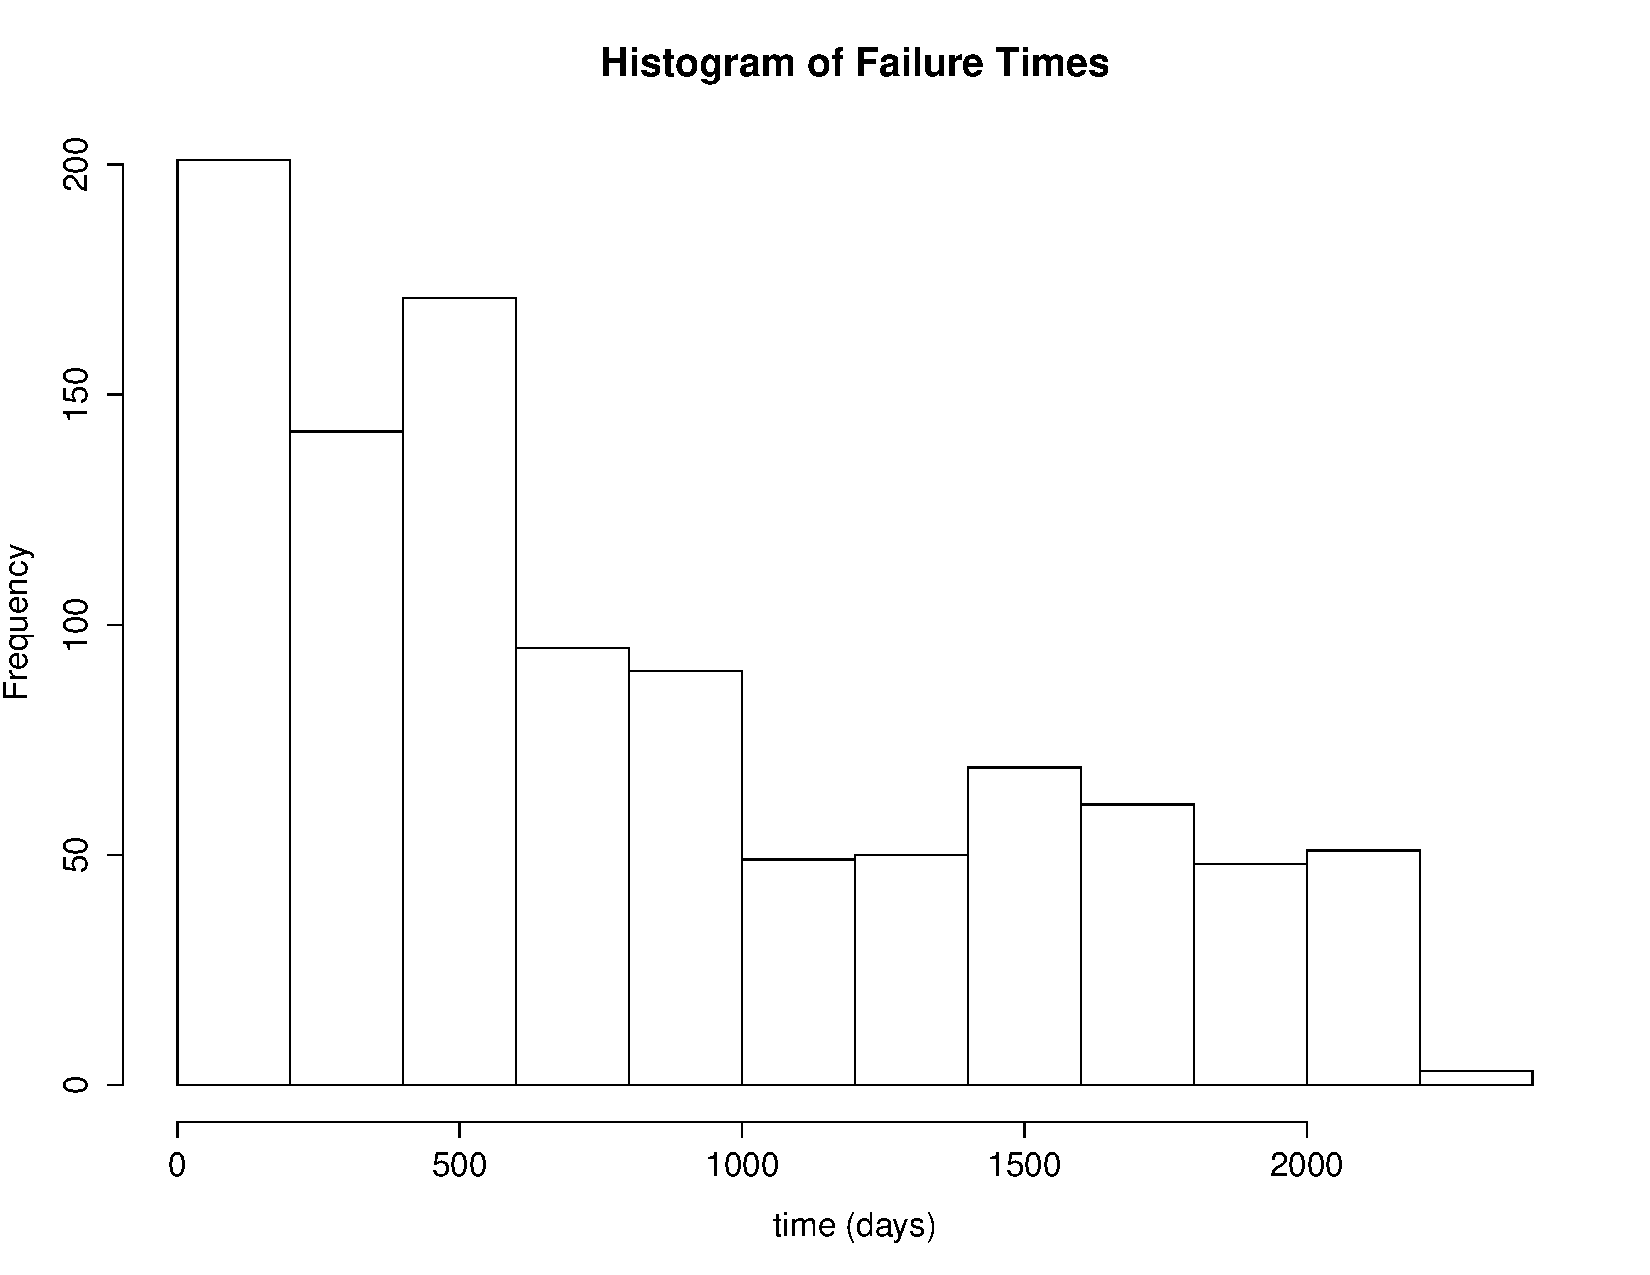
\includegraphics[height=8cm]{failhist.pdf}
\end{figure}
\noindent \textit{Model:}\\\\
We used a Bayesian modeling approach to estimate the Weibull parameters for each model. Rather than modeling each model independently, we modeled the Weibull parameters hierarchically, to pool information and to provide better inferences, particularly for the brands that produced few failures. The model was fit using the rstan package in R \cite{stan}.

We parameterized the Weibull in terms of a lower log quantile, $t_p$ (where $p=0.01$), and scale, $\sigma$. These were modeled by a Student's t with 5 degrees of freedom and a lognormal, respectively.

\[Y_{mi} \stackrel{ind.}{\sim} \operatorname{Weibull}(\eta_m, \beta_m)\]
\[\sigma_m = \frac{1}{\beta_m}, \quad t_{p,m} = \exp\{\log(\eta_m) + \sigma_m \Phi_{sev}(p)\}\]
\[\log(t_{p,m}) \stackrel{i.i.d}{\sim} \operatorname{t}(\nu = 5, \mu_1, \tau_1)\]
\[\sigma_m \stackrel{i.i.d}{\sim} \operatorname{log-normal}(\mu_2, \tau^2_2)\]

The following uninformative and vague priors were used for the hyperparameters.
\[p(\mu_1,\mu_2) \propto 1\]
\[\tau_1,\tau_2 \stackrel{ind.}{\sim} \operatorname{half-Cauchy}(0,10)\]

\noindent \textit{Results:}\\\\
Stan's Hamiltonian MCMC produces posterior distributions for each model's parameters.  Since $\eta$ is extremly far away from the majority of the data we focus on the posterior distribution of $t_p$ (where $p=0.01$) and $\beta$.  The plot below shows the median of the posterior estimate (in hours) along with error bars corresponding to the middle 50\% of the distribution.  Model 2 has the highest time to reach the .01 quatile, while Model 12 is the fastest.  The error bars are commensurate to the number of observations in the data.  Model 11 is the most tested model and has a narrow posterior while Model 2 has a range from about 2,500 to 13,000 hours.
\begin{figure}[H]
\centering
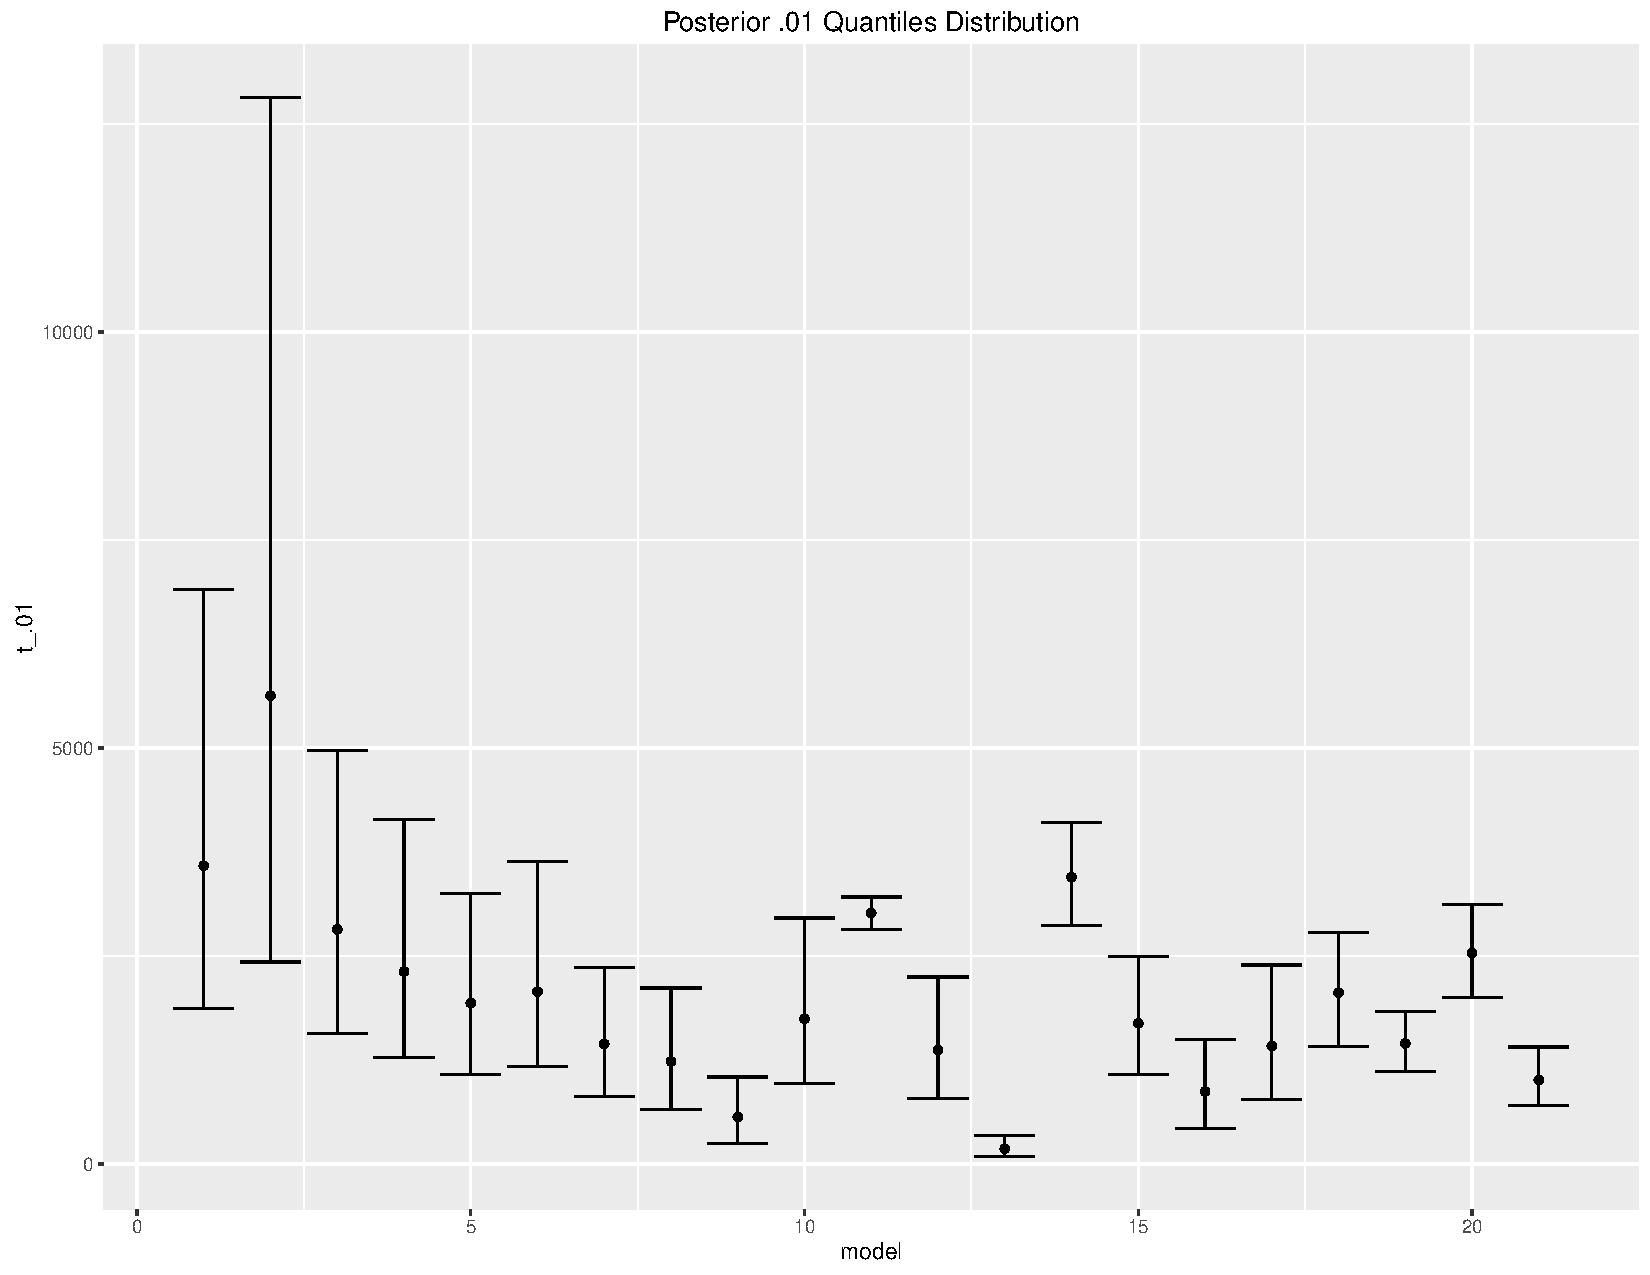
\includegraphics[height=8cm]{postquant.pdf}
\end{figure}

\noindent We can also compare the posteriors of estimated $\beta$ across models.  A line at $\beta=1$ differntiates between models with infant mortality versus those with a hazard that increases over time.  Again, with so few faiures, these results have large margin of errors; however, it does appear that Model 20 has a $\beta$ greater than 1 while Models 1 and 13 have hard drives that suffer from early failures.
\begin{figure}[H]
\centering
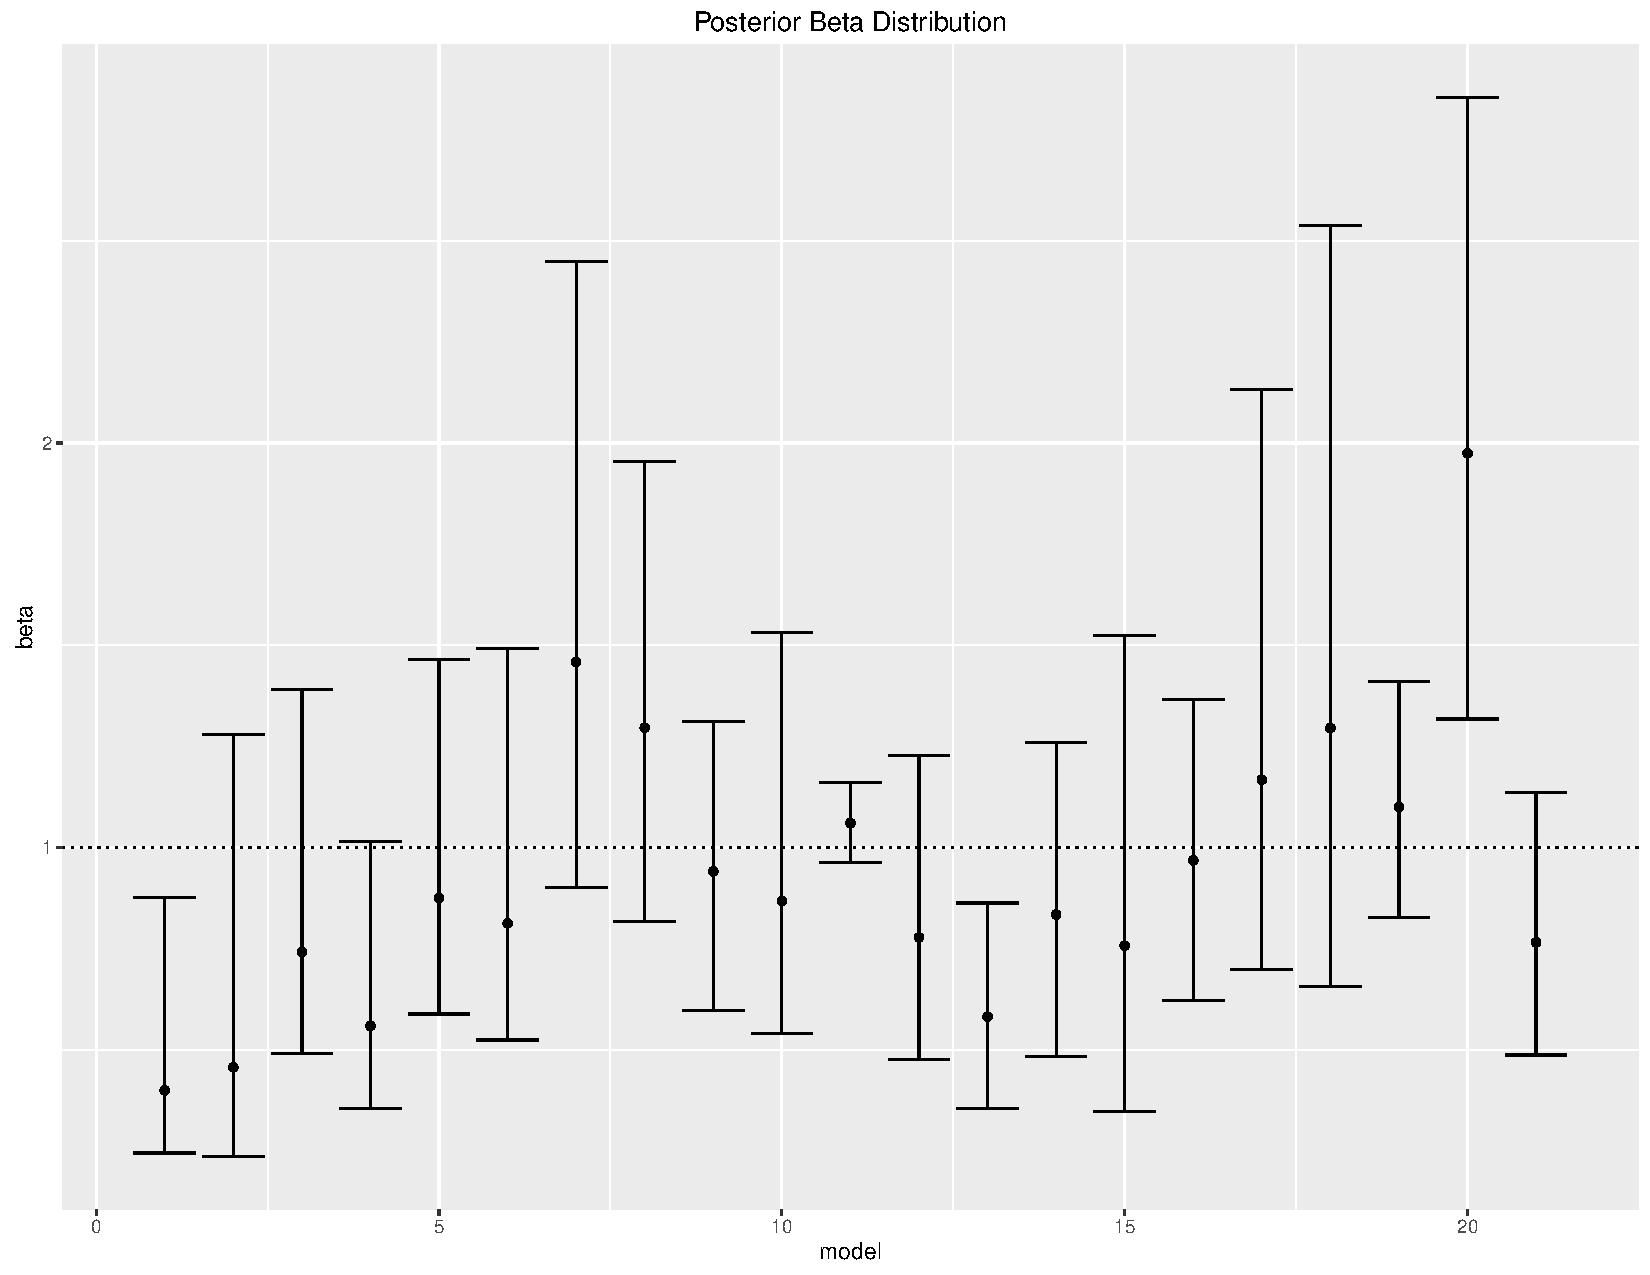
\includegraphics[height=8cm]{postbeta.pdf}
\end{figure}

\noindent Finally, to assess model fit, we overlay the fitted models with an 80\% credible interval ribbon on top of the left truncated adjusted Kaplan-Meier non-parametric estimate.  The emperical CDF is on the y-axis; the x-axis is in terms of hours.  Looking at Model 1 and Model 11 we can see the Weibull model captures the data quite well.  It apperas the credible interval for Model 1 is quite wide; however, the ribbon only covers a narrow range of about .01--and it should be noted that Model 1 only had 22 failures.  In contrast, Model 11 had 381 failures, and as expected the credible interval is thin with the data points hovering in the middle.

\begin{figure}[H]
  \centering
  \begin{minipage}[b]{0.4\textwidth}
    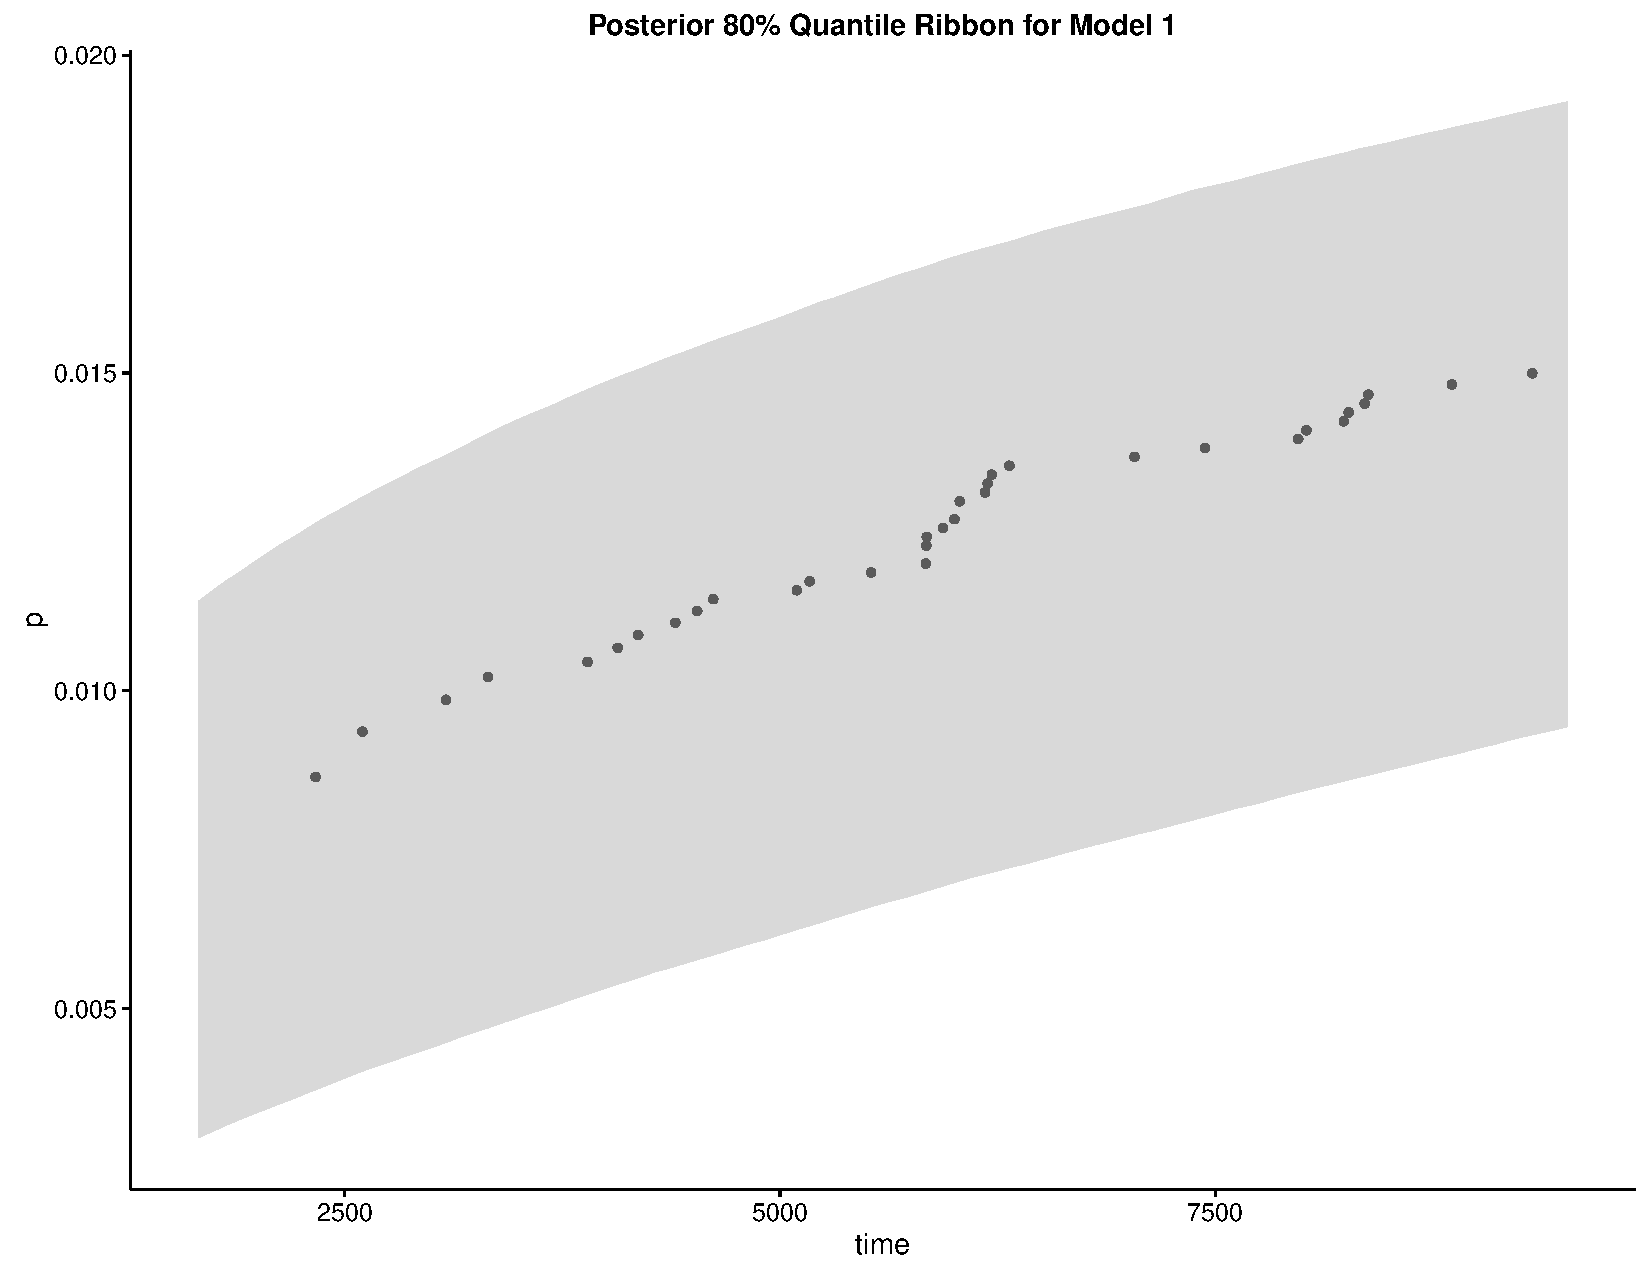
\includegraphics[width=\textwidth]{plot1.pdf}
  \end{minipage}
  \hfill
  \begin{minipage}[b]{0.4\textwidth}
    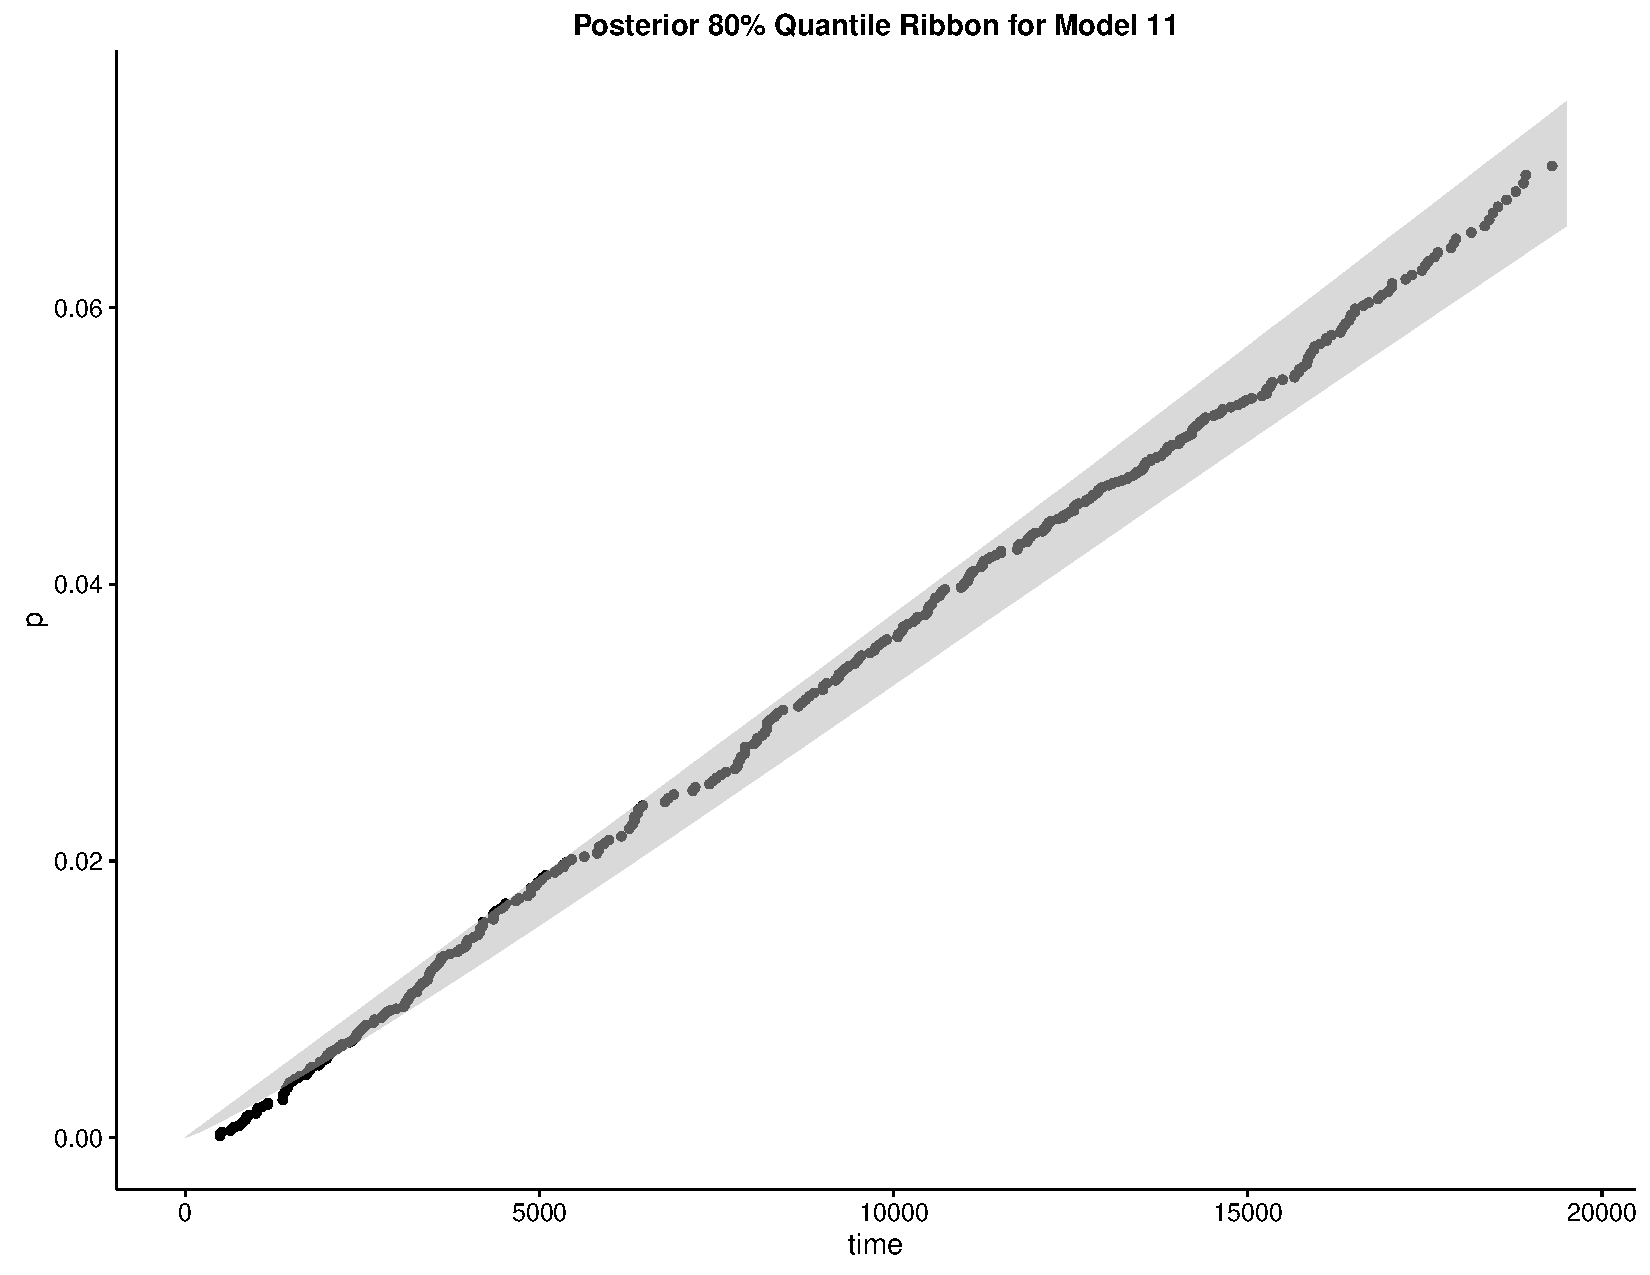
\includegraphics[width=\textwidth]{plot2.pdf}
  \end{minipage}
\end{figure}

\noindent Some hard drive brands were not modeled as well.  Model 15 only had 3 failures and seen below the credible interval does not capture all of the data.  Model 21 had a cluster of failures at around 1000 hours that were not picked up in the model.  Again, though, with only 19 failures there is very little data to accuratly model the failure distribution.  

\begin{figure}[H]
  \centering
  \begin{minipage}[b]{0.4\textwidth}
    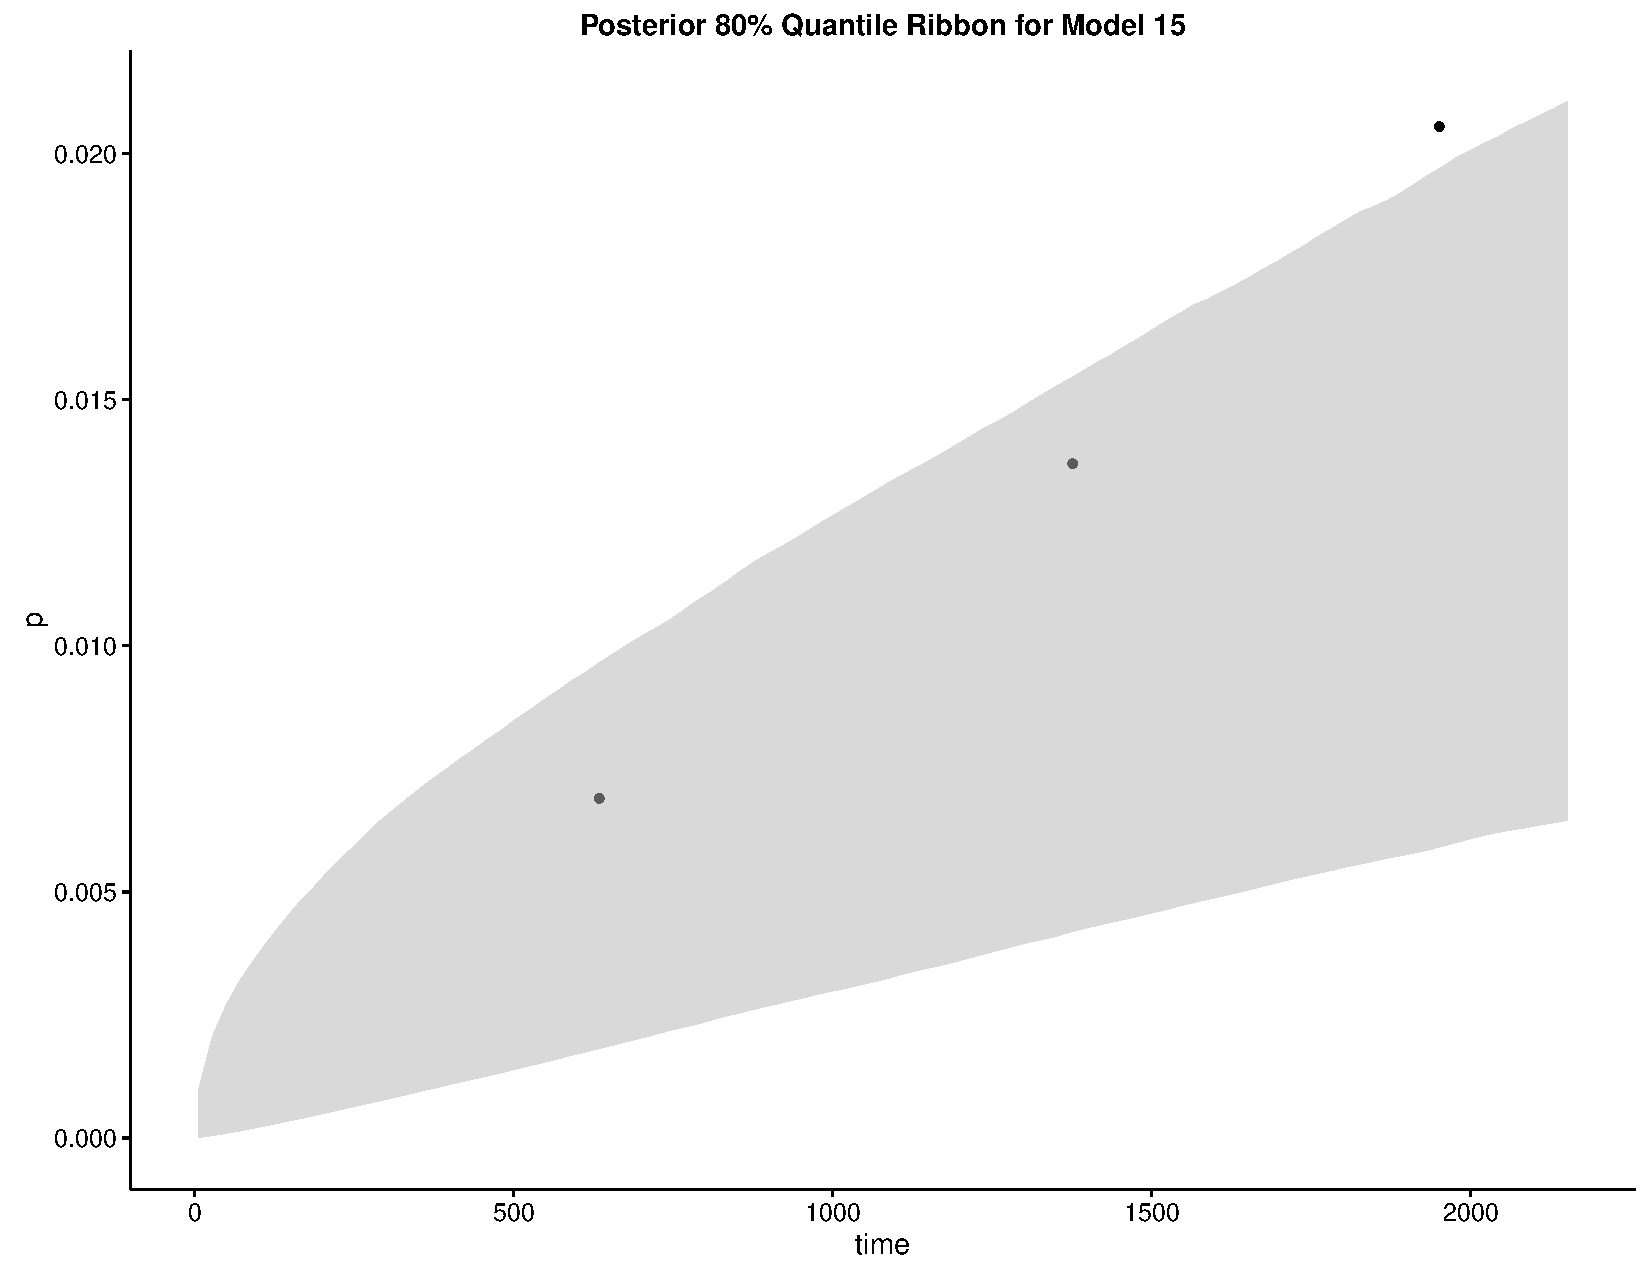
\includegraphics[width=\textwidth]{plot3.pdf}
  \end{minipage}
  \hfill
  \begin{minipage}[b]{0.4\textwidth}
    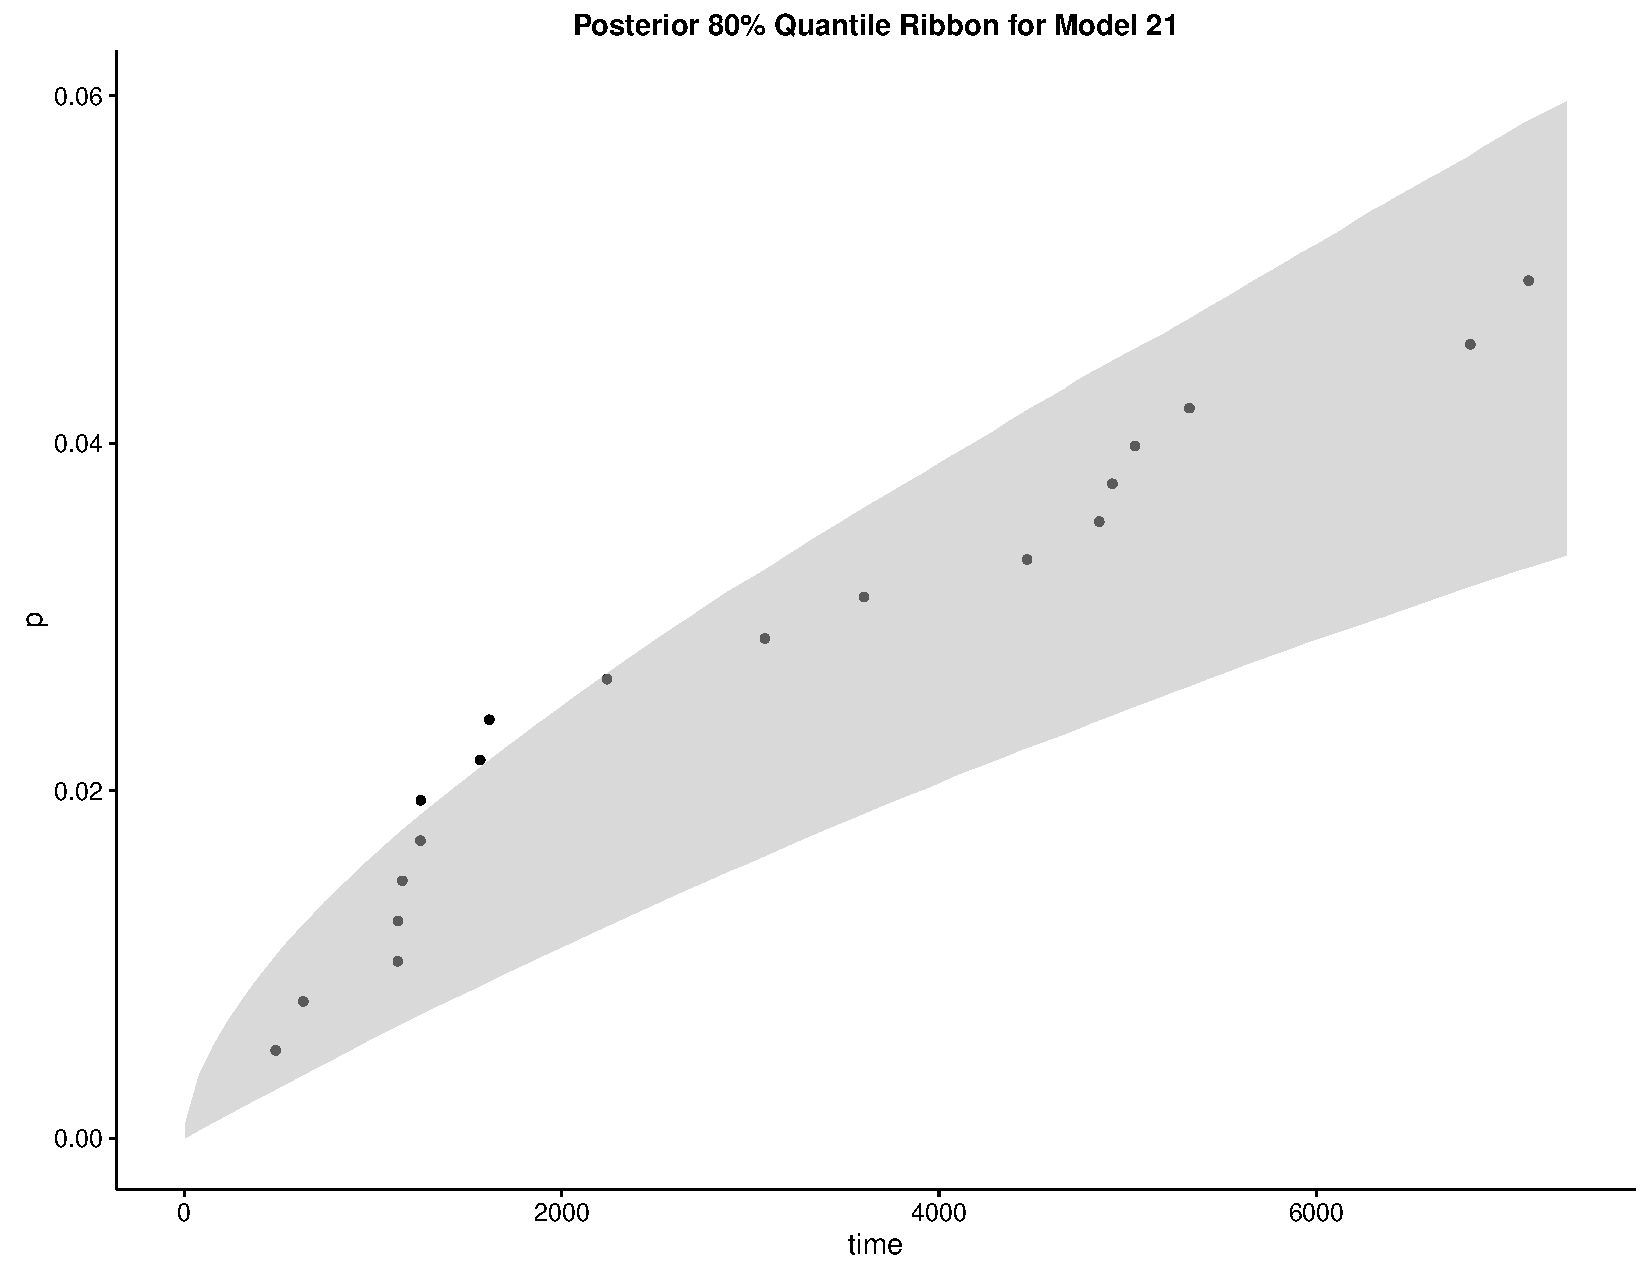
\includegraphics[width=\textwidth]{plot4.pdf}
  \end{minipage}
\end{figure}



\bibliographystyle{plain}
\bibliography{bibliography} 
\clearpage
\begin{appendices}
\section{Stan model:}
{\scriptsize
\begin{verbatim}
data {
  int<lower=0> N_obs;
  int<lower=0> N_cens;
  int<lower=0> N_tr_obs;
  int<lower=0> N_tr_cens;
  int<lower=0> M;

  // right endpoints
  real<lower=0> y_obs[N_obs];
  real<lower=0> y_cens[N_cens];
  real<lower=0> y_tr_obs[N_tr_obs];
  real<lower=0> y_tr_cens[N_tr_cens];

  // truncation points
  real<lower=0> t_obs[N_tr_obs];
  real<lower=0> t_cens[N_tr_cens];

  // explanatory variable
  int<lower=1, upper=M> x_obs[N_obs];
  int<lower=1, upper=M> x_cens[N_cens];
  int<lower=1, upper=M> x_tr_obs[N_tr_obs];
  int<lower=1, upper=M> x_tr_cens[N_tr_cens];

  // quantile to set prior on
  real<lower=0, upper=1> p;
}
transformed data{
  real<lower=0> Q;
  Q <- -1.0 * log(1-p);
}
parameters {
  vector[M] log_tp;
  vector[M] log_sigma;
  real m1;
  real<lower=0> C1;
  real m2;
  real<lower=0> C2;
}
transformed parameters {
  vector<lower=0>[M] eta;
  vector<lower=0>[M] beta;
  beta <- exp(-1.0 * log_sigma);
  for(i in 1:M){
    eta[i] <- exp(log_tp[i])/(Q^(1/beta[i]));
  }
}
model {
  for(i in 1:N_obs){
    y_obs[i] ~ weibull(beta[x_obs[i]], eta[x_obs[i]]);
  }

  for(i in 1:N_cens){
    increment_log_prob(weibull_ccdf_log(y_cens[i], beta[x_cens[i]], eta[x_cens[i]]));
  }

  for(i in 1:N_tr_obs){
    increment_log_prob(        weibull_log(y_tr_obs[i], beta[x_tr_obs[i]], eta[x_tr_obs[i]]));
    increment_log_prob(-1.0 * weibull_ccdf_log(t_obs[i], beta[x_tr_obs[i]], eta[x_tr_obs[i]]));
  }

  for(i in 1:N_tr_cens){
    increment_log_prob(       weibull_ccdf_log(y_tr_cens[i], beta[x_tr_cens[i]], eta[x_tr_cens[i]]));
    increment_log_prob(-1.0 * weibull_ccdf_log(    t_cens[i], beta[x_tr_cens[i]], eta[x_tr_cens[i]]));
  }

  log_tp ~ student_t(5, m1, C1);
  log_sigma ~ normal(m2, C2);

  //priors (improper prior on m1 and m2)
  C1 ~ cauchy(0, 10);
  C2 ~ cauchy(0,10);}
  }
  \end{verbatim}
  }
\end{appendices}

\end{document}

